\documentclass[12pt,titlepage]{article}
\usepackage[margin=1.25in]{geometry}
\usepackage{graphicx,amsmath,blindtext,minted}

%% Variables definition
\newcommand{\vSubject}{Data Structure and Algorithm Practicum}
\newcommand{\vSubtitle}{Linked List}
\newcommand{\vName}{Muhammad Baihaqi Aulia Asy'ari}
\newcommand{\vNIM}{2241720145}
\newcommand{\vClass}{1I}
\newcommand{\vDepartment}{Information Technology}
\newcommand{\vStudyProgram}{D4 Informatics Engineering}

%% [START] Tikz related stuff
\usepackage{tikz}
\usetikzlibrary{svg.path,calc,shapes.geometric,shapes.misc}
\tikzstyle{terminator} = [rectangle, draw, text centered, rounded corners = 1em, minimum height=2em]
\tikzstyle{preparation} = [chamfered rectangle, chamfered rectangle sep=0.75em, draw, text centered, minimum height = 2em]
\tikzstyle{process} = [rectangle, draw, text centered, minimum height=2em]
\tikzstyle{decision} = [diamond, aspect=2, draw, text centered, minimum height=2em]
\tikzstyle{data}=[trapezium, draw, text centered, trapezium left angle=60, trapezium right angle=120, minimum height=2em]
\tikzstyle{connector} = [line width=0.25mm,->]
%% [END] Tikz related stuff

%% [START] Fancy header related stuff
\usepackage{fancyhdr}
\pagestyle{fancy}
\setlength{\headheight}{15pt} % compensate fancyhdr style
\fancyhead{}
\fancyfoot{}
\fancyfoot[L]{\thepage}
\fancyfoot[R]{\textit{\vSubject - \vSubtitle}}
\renewcommand{\footrulewidth}{0.4pt}% default is 0pt, overline for footer
%% [END] Fancy header related stuff

%% [START] Custom tabular command related stuff
\usepackage{tabularx}
\newcommand{\details}[2]{
    #1 & #2  \\
}
%% [END] Custom tabular command related stuff

%% [START] Figure related stuff
\newcommand{\image}[3][1]{
    \begin{figure}[h]
        \centering
        \includegraphics[#1]{#2}
        \caption{#3}
        \label{#3}
    \end{figure}
}
%% [END] Figure related stuff

%%
\usepackage{pgf-umlcd}

\renewcommand{\umldrawcolor}{black}
\renewcommand{\umlfillcolor}{white}
%%

%% [BEGIN] Custom enumerator
\usepackage{enumitem}
%% [END] Custom enumerator

%% [BEGIN] Paragraph indent
\usepackage{indentfirst}
%% [END] Paragraph indent

\begin{document}
\begin{titlepage}
    \centering
    \vfill
    {\bfseries\LARGE
        \vSubject\\
        \vskip0.25cm
        \vSubtitle
    }
    \vfill
    
\includegraphics[width=6cm]{images/polinema-logo.png}
    \vfill
    {
        \textbf{Name}\\
        \vName\\
        \vskip0.5cm
        \textbf{NIM}\\
        \vNIM\\
        \vskip0.5cm
        \textbf{Class}\\
        \vClass\\
        \vskip0.5cm
        \textbf{Department}\\
        \vDepartment\\
        \vskip0.5cm
        \textbf{Study Program}\\
        \vStudyProgram
    }
\end{titlepage}

\newpage

\setcounter{section}{1}
\subsection{Learning Objective}

After learning this practicum, students will be able to:
\begin{enumerate}
    \item Create a linked list data structure
    \item Create a program that implements linked list
    \item Differentiate the problems that can be solved with linked list
\end{enumerate}

\subsection{Lab Activities 1}
In this practicum, we will implement how to create single linked list with nodes data representation, accessing the linked list, and adding the data.

\subsubsection{Steps}
\begin{enumerate}
    \item Create a new package named \textbf{week11}
    \item Add these following classes:

    \begin{enumerate}
        \item Node.java
        \item SingleLinkedList.java
        \item SLLMain.java
    \end{enumerate}

    \item Create Node class
    \begin{minted}[autogobble,breaklines]{java}
        package labActivities;

        public class Node {
            int data;
            Node next;

            public Node(int data, Node next) {
                this.data = data;
                this.next = next;
            }
        }
    \end{minted}
    \item Add these following attributes in class \textbf{SingleLinkedList}
    \begin{minted}[autogobble,breaklines]{java}
        public class SingleLinkedList {
            Node head;
            Node tail;
        }
    \end{minted}
    \item For the next step, we will implement methods that are exist in \textbf{SingleLinkedList}
    \begin{minted}[autogobble,breaklines]{java}
        public class SingleLinkedList {
            Node head;
            Node tail;
        }
    \end{minted}
    \item Add method isEmpty()
    \begin{minted}[autogobble,breaklines]{java}
        public boolean isEmpty() {
            return head == null;
        }
    \end{minted}
    \item Implement this method to display the data with traverse process
    \begin{minted}[autogobble,breaklines]{java}
        public void print() {
            if (!isEmpty()) {
                Node tmp = head;
                System.out.print("Linked list content: \t");
                while (tmp != null) {
                    System.out.print(tmp.data + "\t");
                    tmp = tmp.next;
                }
                System.out.println("");
            } else {
                System.out.println("Linked list is empty");
            }
        }
    \end{minted}
    \item Implement method \textbf{addFirst()}
    \begin{minted}[autogobble,breaklines]{java}
        public void addFirst(int input) {
            Node ndInput = new Node(input, null);
            if (isEmpty()) {
                head = ndInput;
                tail = ndInput;
            } else {
                ndInput.next = head;
                head = ndInput;
            }
        }
    \end{minted}
    \item Implement method \textbf{addLast()}
    \begin{minted}[autogobble,breaklines]{java}
        public void addLast(int input) {
            Node ndInput = new Node(input, null);
            if (isEmpty()) {
                head = ndInput;
                tail = ndInput;
            } else {
                tail.next = ndInput;
                tail = ndInput;
            }
        }
    \end{minted}
    \item Implement method \textbf{insertAfter()}, to insert a node that stores data that were inputted by the user after data \textbf{key}
    \begin{minted}[autogobble,breaklines]{java}
        public void insertAfter(int key, int input) {
            Node ndInput = new Node(input, null);
            Node temp = head;
            do {
                if (temp.data == key) {
                    ndInput.next = temp.next;
                    temp.next = ndInput;
                    if (ndInput.next == null) tail = ndInput;
                    break;
                }
                temp = temp.next;
            } while (temp != null);
        }
    \end{minted}
    \item Add these following codes to add a node based on defined index
    \begin{minted}[autogobble,breaklines]{java}
        public void insertAt(int index, int input) {
            if (index < 0) {
                System.out.println("Wrong index");
            } else if (index == 0) {
                addFirst(input);
            } else {
                Node temp = head;
                for (int i = 0; i < index - 1; i++) {
                    temp = temp.next;
                }
                temp.next = new Node(input, temp.next);
                if (temp.next.next == null) tail = temp.next;
            }
        }
    \end{minted}
    \item In class \textbf{SLLMain}, create main function and instantiate a new object from \textbf{SingleLinkedList} class
    \begin{minted}[autogobble,breaklines]{java}
        public class SLLMain {
            public static void main(String[] args) {
                SingleLinkedList singLL = new SingleLinkedList();
            }
        }
    \end{minted}
    \item Add methods for inserting data, as well as displaying the data for each insert process so that we can track the changes
    \begin{minted}[autogobble,breaklines]{java}
        singLL.print();
        singLL.addFirst(890);
        singLL.print();
        singLL.addLast(760);
        singLL.print();
        singLL.addFirst(700);
        singLL.print();
        singLL.insertAfter(700, 999);
        singLL.print();
        singLL.insertAt(3, 833);
        singLL.print();
    \end{minted}
\end{enumerate}

\subsubsection{Result}

\begin{minted}[autogobble,breaklines,linenos]{text}
    PS D:\Kuliah\Smt 2\Algoritma dan Struktur Data\Praktikum\Week 11\Linked List>  & 'C:\Program Files\Java\jdk-18.0.2.1\bin\java.exe' '-XX:+ShowCodeDetailsInExceptionMessages' '-cp' 'D:\Kuliah\Smt 2\Algoritma dan Struktur Data\Praktikum\Week 11\Linked List\bin' 'labActivities.SLLMain'
    Linked list is empty
    Linked list content:    890
    Linked list content:    890     760
    Linked list content:    700     890     760
    Linked list content:    700     999     890     760
    Linked list content:    700     999     890     833     760
\end{minted}

\subsubsection{Question}

\begin{enumerate}
    \item Why the output of the program in first line is “Linked list is empty”?
    \item Please explain the usage of these following codes in:
    \begin{minted}[autogobble,breaklines]{java}
        ndInput.next = temp.next;
        temp.next = ndInput;
    \end{minted}
    \item In \textbf{SingleLinkedList}, what is the usage of this following code in \textbf{insertAt}?
    \begin{minted}[autogobble,breaklines]{java}
        if (temp.next.next == null) tail =  temp.next;
    \end{minted} 
\end{enumerate}

\subsection{Lab Activities 2}
In this practicum, we will try to learn and implement how to access node elements, get index, and node removal in a Single Linked List

\subsubsection{Steps}
\begin{enumerate}
    \item Implement methods to access data and index in linked list
    \item Add methods to get data based on certain index from class \textbf{SingleLinkedList}
    \begin{minted}[autogobble,breaklines]{java}
        public int getData(int index) {
            Node temp = head;
            for (int i = 0; i < index; i++) {
                temp = temp.next;
            }
            return temp.data;
        }
    \end{minted}
    \item Implement method \textbf{indexOf}
    \begin{minted}[autogobble,breaklines]{java}
        public int indexOf(int key) {
            Node temp = head;
            int index = 0;
            while (temp != null && temp.data != key) {
                temp = temp.next;
                index++;
            }

            if (temp == null) {
                return -1;
            } else {
                return index;
            }
        }
    \end{minted}
    \item Add method \textbf{removeFirst()} in class \textbf{SingleLinkedList}
    \begin{minted}[autogobble,breaklines]{java}
        public void removeFirst() {
            if (isEmpty()) {
                System.out.println("Linked list is empty. Can not remove data");
            } else if (head == tail) {
                head = tail = null;
            } else {
                head = head.next;
            }
        }
    \end{minted}
    \item Add this method to remove data that is in the last of the list from class \textbf{SingleLinkedList}
    \begin{minted}[autogobble,breaklines]{java}
        public void removeLast() {
            if (isEmpty()) {
                System.out.println("Linked list is empty. Can not remove data");
            } else if (head == tail) {
                head = tail = null;
            } else {
                Node temp = head;
                while (temp.next != tail) {
                    temp = temp.next;
                }
                temp.next = null;
                tail = temp;
            }
        }
    \end{minted}
    \item Next, we will implement method \textbf{remove()}
    \begin{minted}[autogobble,breaklines]{java}
        public void remove(int key) {
            if (isEmpty()) {
                System.out.println("Linked list is empty. Can not remove data");
            } else {
                Node temp = head;
                while (temp != null) {
                    if (temp.data == key && temp == head) {
                        this.removeFirst();
                        break;
                    } else if (temp.next.data == key) {
                        temp.next = temp.next.next;
                        if (temp.next == null) {
                            tail = temp;
                        }
                        break;
                    }
                    temp = temp.next;
                }
            }
        }
    \end{minted}
    \item Create a method to remove a node based on defined index
    \begin{minted}[autogobble,breaklines]{java}
        public void removeAt(int index) {
            if (index == 0) {
                removeFirst();
            } else {
                Node temp = head;
                for (int i = 0; i < index; i++) {
                    temp = temp.next;
                }
                temp.next = temp.next.next;
                if (temp.next == null) {
                    tail = temp;
                }
            }
        }
    \end{minted}
    \item Next, we will try to access and remove data in main method in class \textbf{SLLMain} by adding these codes
    \begin{minted}[autogobble,breaklines]{java}
        System.out.println("Data in the 1st index : " + singLL.getData(1));
        System.out.println("Data 3 is in index : " + singLL.indexOf(760));
        singLL.remove(999);
        singLL.print();
        singLL.removeAt(0);
        singLL.print();
        singLL.removeFirst();
        singLL.print();
        singLL.removeLast();
        singLL.print();
    \end{minted}
    \item Method \textbf{SLLMain} becomes like this:
    \begin{minted}[autogobble,breaklines]{java}
        public class SLLMain {
            public static void main(String[] args) {
                SingleLinkedList singLL = new SingleLinkedList();

                singLL.print();
                singLL.addFirst(890);
                singLL.print();
                singLL.addLast(760);
                singLL.print();
                singLL.addFirst(700);
                singLL.print();
                singLL.insertAfter(700, 999);
                singLL.print();
                singLL.insertAt(3, 833);
                singLL.print();

                System.out.println("Data in the 1st index : " + singLL.getData(1));
                System.out.println("Data 3 is in index : " + singLL.indexOf(760));
                singLL.remove(999);
                singLL.print();
                singLL.removeAt(0);
                singLL.print();
                singLL.removeFirst();
                singLL.print();
                singLL.removeLast();
                singLL.print();
            }
        }
    \end{minted}
    \item Execute the class \textbf{SLLMain}
\end{enumerate}

\subsubsection{Result}
\begin{minted}[autogobble,breaklines]{text}
    PS D:\Kuliah\Smt 2\Algoritma dan Struktur Data\Praktikum\Week 11\Linked List>  d:; cd 'd:\Kuliah\Smt 2\Algoritma dan Struktur Data\Praktikum\Week 11\Linked List'; & 'C:\Program Files\Java\jdk-18.0.2.1\bin\java.exe' '-XX:+ShowCodeDetailsInExceptionMessages' '-cp' 'D:\Kuliah\Smt 2\Algoritma dan Struktur Data\Praktikum\Week 11\Linked List\bin' 'labActivities.SLLMain' 
    Linked list is empty
    Linked list content:    890
    Linked list content:    890     760
    Linked list content:    700     890     760
    Linked list content:    700     999     890     760
    Linked list content:    700     999     890     833     760
    Data in the 1st index : 999
    Data 3 is in index : 4
    Linked list content:    700     890     833     760
    Linked list content:    890     833     760
    Linked list content:    833     760
    Linked list content:    833
\end{minted}

\subsubsection{Question}
\begin{enumerate}
    \item Why we use \textbf{break} keyword in remove function? Please explain
    \item Please explain why we implement these following codes in method remove
    \begin{minted}[autogobble,breaklines]{java}
        else if (temp.next.data == key) {
            temp.next = temp.next.next;
        }
    \end{minted}
    \item What are the outputs of method indexOf? Please explain each of the output!
\end{enumerate}

\subsection{Assignments}
\begin{enumerate}
    \item Create a method \textbf{insertBefore()} to add node before the desired keyword
    \begin{minted}[autogobble,breaklines]{java}
        public void insertBefore(int key, int input) {
            Node ndInput = new Node(input, null);
            if (isEmpty()) {
                head = tail = ndInput;
            } else if (head.equals(tail)) {
                ndInput.next = head;
                head = ndInput;
            } else {
                Node temp = head;
                while (!temp.next.equals(null)) {
                    if (temp.next.data == key) {
                        temp.next = new Node(input, temp.next);
                    }
                    temp = temp.next;
                }
            }
        }
    \end{minted}
    \item Implement the linked list from this following image. You may use \textbf{4} method of adding data we’ve learnt
    \hbox{}\\
    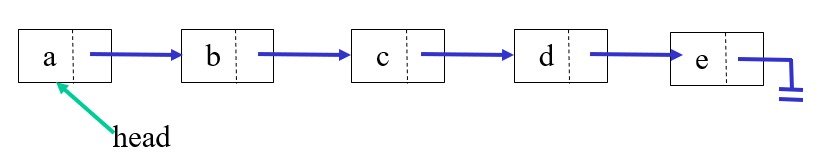
\includegraphics[width=\textwidth]{images/figures/fig1.jpeg}
    \texttt{Node.java}
    \begin{minted}[autogobble,breaklines]{java}
        package assignment;

        public class Node {
            String data;
            Node next;

            public Node(String data, Node next) {
                this.data = data;
                this.next = next;
            }
        }
    \end{minted}
    \texttt{SingleLinkedList.java}
    \begin{minted}[autogobble,breaklines]{java}
        package assignment;

        public class SingleLinkedList {
            Node head;
            Node tail;

            public boolean isEmpty() {
                return head == null;
            }

            public void print() {
                if (!isEmpty()) {
                    Node tmp = head;
                    System.out.print("Linked list content: \t");
                    while (tmp != null) {
                        System.out.print(tmp.data + "\t");
                        tmp = tmp.next;
                    }
                    System.out.println("");
                } else {
                    System.out.println("Linked list is empty");
                }
            }

            public void addFirst(String input) {
                Node ndInput = new Node(input, null);
                if (isEmpty()) {
                    head = ndInput;
                    tail = ndInput;
                } else {
                    ndInput.next = head;
                    head = ndInput;
                }
            }

            public void addLast(String input) {
                Node ndInput = new Node(input, null);
                if (isEmpty()) {
                    head = ndInput;
                    tail = ndInput;
                } else {
                    tail.next = ndInput;
                    tail = ndInput;
                }
            }

            public void insertAfter(String key, String input) {
                Node ndInput = new Node(input, null);
                Node temp = head;
                do {
                    if (temp.data.equals(key)) {
                        ndInput.next = temp.next;
                        temp.next = ndInput;
                        if (ndInput.next.equals(null)) tail = ndInput;
                        break;
                    }
                    temp = temp.next;
                } while (!temp.equals(null));
            }

            public void insertAt(int index, String input) {
                if (index < 0) {
                    System.out.println("Wrong index");
                } else if (index == 0) {
                    addFirst(input);
                } else {
                    Node temp = head;
                    for (int i = 0; i < index - 1; i++) {
                        temp = temp.next;
                    }
                    temp.next = new Node(input, temp.next);
                    if (temp.next.next.equals(null)) tail = temp.next;
                }
            }

            public String getData(int index) {
                Node temp = head;
                for (int i = 0; i < index; i++) {
                    temp = temp.next;
                }
                return temp.data;
            }

            public int indexOf(String key) {
                Node temp = head;
                int index = 0;
                while (!temp.equals(null) && !temp.data.equals(key)) {
                    temp = temp.next;
                    index++;
                }
                if (temp.equals(null)) {
                    return -1;
                } else {
                    return index;
                }
            }

            public void removeFirst() {
                if (isEmpty()) {
                    System.out.println("Linked list is empty. Can not remove data");
                } else if (head.equals(tail)) {
                    head = tail = null;
                } else {
                    head = head.next;
                }
            }

            public void removeLast() {
                if (isEmpty()) {
                    System.out.println("Linked list is empty. Can not remove data");
                } else if (head.equals(tail)) {
                    head = tail = null;
                } else {
                    Node temp = head;
                    while (!temp.next.equals(tail)) {
                        temp = temp.next;
                    }
                    temp.next = null;
                    tail = temp;
                }
            }

            public void remove(String key) {
                if (isEmpty()) {
                    System.out.println("Linked list is empty. Can not remove data");
                } else {
                    Node temp = head;
                    while (!temp.equals(null)) {
                        if (temp.data.equals(key) && temp.equals(head)) {
                            this.removeFirst();
                            break;
                        } else if (temp.next.data.equals(key)) {
                            temp.next = temp.next.next;
                            if (temp.next == null) {
                                tail = temp;
                            }
                            break;
                        }
                        temp = temp.next;
                    }
                }
            }

            public void removeAt(int index) {
                if (index == 0) {
                    removeFirst();
                } else {
                    Node temp = head;
                    for (int i = 0; i < index; i++) {
                        temp = temp.next;
                    }
                    temp.next = temp.next.next;
                    if (temp.next.equals(null)) {
                        tail = temp;
                    }
                }
            }

            public void insertBefore(String key, String input) {
                Node ndInput = new Node(input, null);
                if (isEmpty()) {
                    head = tail = ndInput;
                } else if (head.equals(tail)) {
                    ndInput.next = head;
                    head = ndInput;
                } else {
                    Node temp = head;
                    while (!temp.next.equals(null)) {
                        if (temp.next.data.equals(key)) {
                            temp.next = new Node(input, temp.next);
                        }
                        temp = temp.next;
                    }
                }
            }
        }
    \end{minted}
    \texttt{SLLMain.java}
    \begin{minted}[autogobble,breaklines]{java}
        package assignment;

        public class SLLMain {
            public static void main(String[] args) {
                SingleLinkedList singLL = new SingleLinkedList();
            
                singLL.addFirst("a");
                singLL.addLast("e");
                singLL.insertAt(1, "b");
                singLL.insertAfter("b", "c");
                singLL.insertAfter("c", "d");
                singLL.print();
            }
        }
    \end{minted}
    \item Create this following \textbf{Stack} implementation using Linked List implementation
    \hbox{}\\
    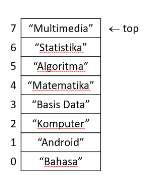
\includegraphics[width=.2\textwidth]{images/figures/fig2.jpeg}
    \includegraphics[width=.8\textwidth]{images/figures/fig3invert.jpg}
    \texttt{Stack.java}
    \begin{minted}[autogobble,breaklines]{java}
        package assignment;

        public class Stack {
            private final SingleLinkedList singLL = new SingleLinkedList();

            public void push(String data) {
                singLL.addFirst(data);
            }

            public String pop() {
                String data = singLL.getData(0);
                singLL.removeFirst();
                return data;
            }

            public void print() {
                singLL.print();
            }
        }
    \end{minted}
    \texttt{StackMain.java}
    \begin{minted}[autogobble,breaklines]{java}
        package assignment;

        public class StackMain {
            public static void main(String[] args) {
                Stack stack = new Stack();

                String[] data = {"Bahasa", "Android", "Komputer", "Basis Data", "Matematika", "Algoritma", "Statistika", "Multimedia"};

                for (int i = 0; i < data.length; i++) {
                    stack.push(data[i]);
                }

                stack.print();
            }
        }
    \end{minted}
    \item Create a program that helps bank customer using linked list with data are as follows: Name, address, and customerAccountNumber
    \texttt{Customer.java}
    \begin{minted}[autogobble,breaklines]{java}
        package assignment;

        public class Customer {
            String name,
            address,
            customerAccountNumber;

            public Customer(String name, String address, String customerAccountNumber) {
                this.name = name;
                this.address = address;
                this.customerAccountNumber = customerAccountNumber;
            }
        }
    \end{minted}
    \item Implement \textbf{Queue} in previous number with \textbf{linked list} concept
    \texttt{Customer.java}
    \begin{minted}[autogobble,breaklines]{java}
        package assignment;

        public class Customer {
            String name,
            address,
            customerAccountNumber;

            public Customer(String name, String address, String customerAccountNumber) {
                this.name = name;
                this.address = address;
                this.customerAccountNumber = customerAccountNumber;
            }

            public void print() {
                System.out.println("================");
                System.out.println("Name: " + name);
                System.out.println("Address: " + address);
                System.out.println("Account Number: " + customerAccountNumber);
            }
        }
    \end{minted}
    \texttt{NodeCustomer.java}
    \begin{minted}[autogobble,breaklines]{java}
        package assignment;

        public class NodeCustomer {
            Customer data;
            NodeCustomer next;

            public NodeCustomer(Customer data, NodeCustomer next) {
                this.data = data;
                this.next = next;
            }
        }
    \end{minted}
    \texttt{SingleLinkedListCustomer.java}
    \begin{minted}[autogobble,breaklines]{java}
        package assignment;

        public class SingleLinkedListCustomer {
            NodeCustomer head;
            NodeCustomer tail;

            public boolean isEmpty() {
                return head == null;
            }

            public void print() {
                if (!isEmpty()) {
                    NodeCustomer tmp = head;
                    System.out.print("Linked list content: \t");
                    while (tmp != null) {
                        System.out.print(tmp.data + "\t");
                        tmp = tmp.next;
                    }
                    System.out.println("");
                } else {
                    System.out.println("Linked list is empty");
                }
            }

            public void addFirst(Customer input) {
                NodeCustomer ndInput = new NodeCustomer(input, null);
                if (isEmpty()) {
                    head = ndInput;
                    tail = ndInput;
                } else {
                    ndInput.next = head;
                    head = ndInput;
                }
            }

            public void addLast(Customer input) {
                NodeCustomer ndInput = new NodeCustomer(input, null);
                if (isEmpty()) {
                    head = ndInput;
                    tail = ndInput;
                } else {
                    tail.next = ndInput;
                    tail = ndInput;
                }
            }

            public void insertAfter(Customer key, Customer input) {
                NodeCustomer ndInput = new NodeCustomer(input, null);
                NodeCustomer temp = head;
                do {
                    if (temp.data.equals(key)) {
                        ndInput.next = temp.next;
                        temp.next = ndInput;
                        if (ndInput.next.equals(null)) tail = ndInput;
                        break;
                    }
                    temp = temp.next;
                } while (!temp.equals(null));
            }

            public void insertAt(int index, Customer input) {
                if (index < 0) {
                    System.out.println("Wrong index");
                } else if (index == 0) {
                    addFirst(input);
                } else {
                    NodeCustomer temp = head;
                    for (int i = 0; i < index - 1; i++) {
                        temp = temp.next;
                    }
                    temp.next = new NodeCustomer(input, temp.next);
                    if (temp.next.next.equals(null)) tail = temp.next;
                }
            }

            public Customer getData(int index) {
                NodeCustomer temp = head;
                for (int i = 0; i < index; i++) {
                    temp = temp.next;
                }
                return temp.data;
            }

            public int indexOf(String key) {
                NodeCustomer temp = head;
                int index = 0;
                while (!temp.equals(null) && !temp.data.equals(key)) {
                    temp = temp.next;
                    index++;
                }
                if (temp.equals(null)) {
                    return -1;
                } else {
                    return index;
                }
            }

            public void removeFirst() {
                if (isEmpty()) {
                    System.out.println("Linked list is empty. Can not remove data");
                } else if (head.equals(tail)) {
                    head = tail = null;
                } else {
                    head = head.next;
                }
            }

            public void removeLast() {
                if (isEmpty()) {
                    System.out.println("Linked list is empty. Can not remove data");
                } else if (head.equals(tail)) {
                    head = tail = null;
                } else {
                    NodeCustomer temp = head;
                    while (!temp.next.equals(tail)) {
                        temp = temp.next;
                    }
                    temp.next = null;
                    tail = temp;
                }
            }

            public void remove(String key) {
                if (isEmpty()) {
                    System.out.println("Linked list is empty. Can not remove data");
                } else {
                    NodeCustomer temp = head;
                    while (!temp.equals(null)) {
                        if (temp.data.equals(key) && temp.equals(head)) {
                            this.removeFirst();
                            break;
                        } else if (temp.next.data.equals(key)) {
                            temp.next = temp.next.next;
                            if (temp.next == null) {
                                tail = temp;
                            }
                            break;
                        }
                        temp = temp.next;
                    }
                }
            }

            public void removeAt(int index) {
                if (index == 0) {
                    removeFirst();
                } else {
                    NodeCustomer temp = head;
                    for (int i = 0; i < index; i++) {
                        temp = temp.next;
                    }
                    temp.next = temp.next.next;
                    if (temp.next.equals(null)) {
                        tail = temp;
                    }
                }
            }

            public void insertBefore(Customer key, Customer input) {
                NodeCustomer ndInput = new NodeCustomer(input, null);
                if (isEmpty()) {
                    head = tail = ndInput;
                } else if (head.equals(tail)) {
                    ndInput.next = head;
                    head = ndInput;
                } else {
                    NodeCustomer temp = head;
                    while (!temp.next.equals(null)) {
                        if (temp.next.data.equals(key)) {
                            temp.next = new NodeCustomer(input, temp.next);
                        }
                        temp = temp.next;
                    }
                }
            }
        }
    \end{minted}
    \texttt{Queue.java}
    \begin{minted}[autogobble,breaklines]{java}
        package assignment;

        public class Queue {
            private final SingleLinkedListCustomer list = new SingleLinkedListCustomer();

            public void enqueue(Customer data) {
                list.addLast(data);
            }

            public Customer dequeue() {
                    Customer data = list.getData(0);
                    list.removeFirst();
                    return data;
            }

            public void print() {
                NodeCustomer temp = list.head;
                while (temp != null) {
                    temp.data.print();
                    temp = temp.next;
                }
            }
        }
    \end{minted}
\end{enumerate}

\end{document}